% Nama Kelompok : Kelompok 2
% Kelas : D4 TI 1A
% 1. Kadek Diva Krishna Murti (1174006)
% 2. Duvan Silalahi (1174011)
% 3. Oniwaldus (1174005)
% 4. Choirul Anam (1174004)
% 5. Sri Rahayu (1174015)
% 6. Ilham Habibi (1174028)

\section{Pengertiani}


IDE merupakan singkatan dari Integrated Development Environment atau lingkungan terintegrasi yang digunakan untuk melakukan pengembangan. Dikatakan sebagai lingkungan karena melalui software inilah dilakukan pemrograman Arduino untuk melakukan fungsi - fungsi yang ditanamkan melalui sintaks pemrograman. IDE ini disediakan gratis dan bisa didapatkan secara langsung pada halaman resmi arduino yang bersifat        
\subsection{New}
New berfungsi untuk membuat Sketch baru.
\subsection{Open}
Open berfungsi untuk membuka kembali sketch yang telah dibuat sebelumnya untuk dilakukan perubahan atau hanya diupload ulang ke Arduino.










%%%%TARUH DIATAS JANGAN TARUH DIATAS%%%%%
%%%%%%%%%%%%%%%%%%%%%%%%%%%%%%%%%%%%%%%%%%%%%%%%%%%%%%%%%%
\section{Proses Instalasi}

\begin{enumerate}
\item Pertama unduh terlebih dahulu installer IDE Arduino di https://www.arduino.cc/en/Main/Software. Pada halaman tersebut ada tiga macam installer yang dapat diunduh sesuai dengan Operating System yang kita pakai.
\break
\centerline{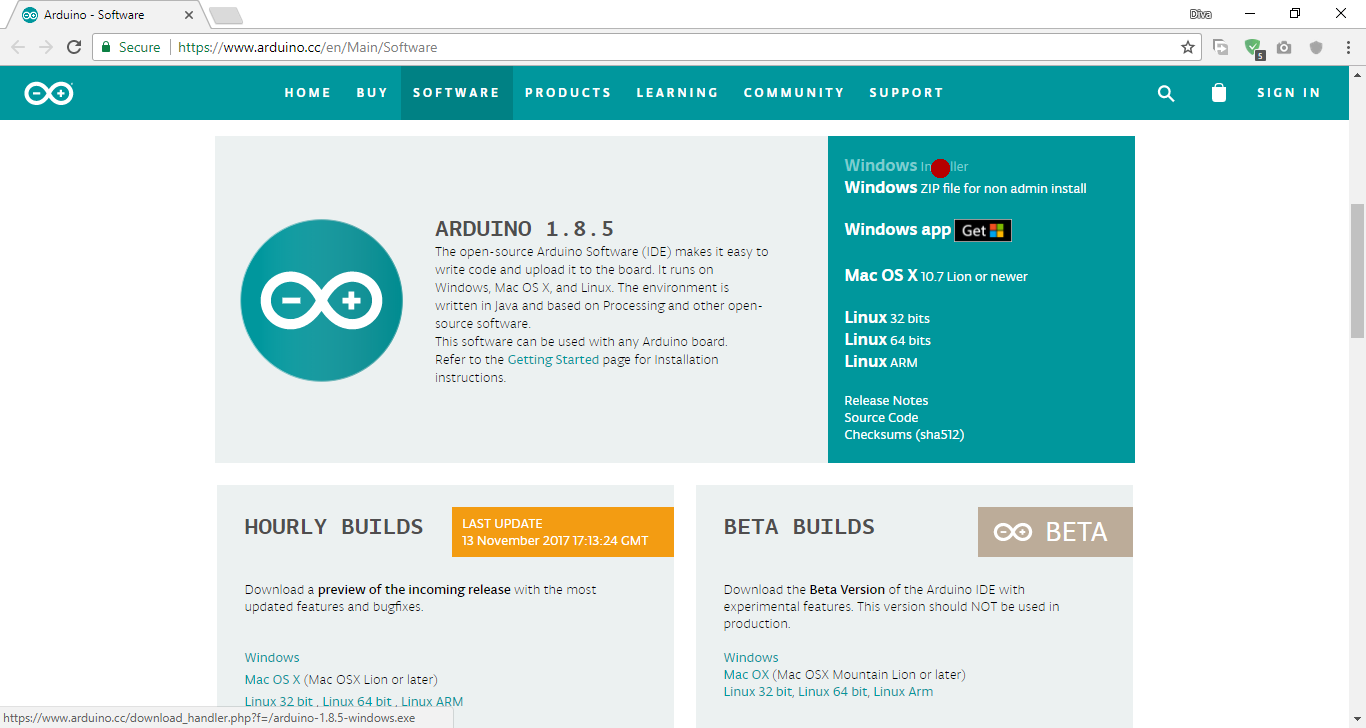
\includegraphics[width=0.9\textwidth]{figures/aride8.png}}
\item Kemudian pada halaman tersebut ada dua pilihan apakah kita ingin berkontribusi dengan memberikan uang sesuai dengan nominal yang tertera atau hanya mengunduh saja. Disini kita klik `Just Download' dan proses mengunduh dimulai.
\break
\centerline{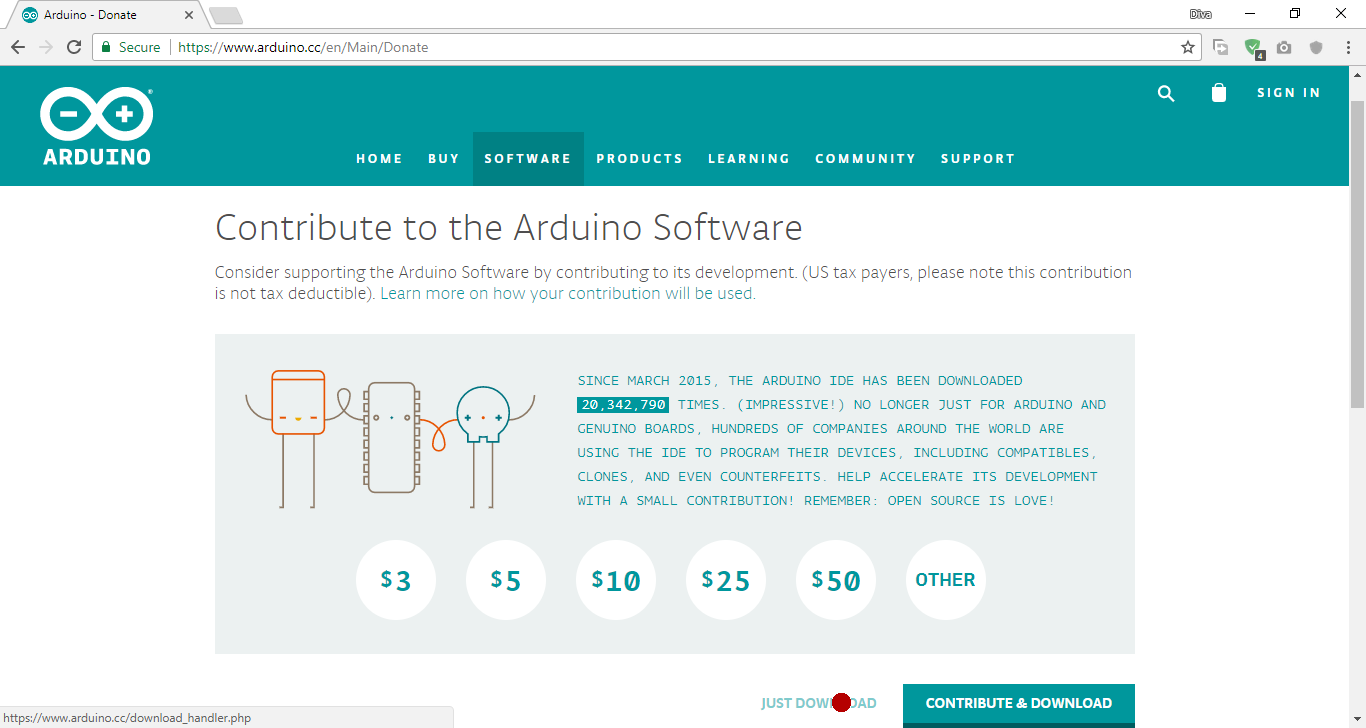
\includegraphics[width=0.9\textwidth]{figures/aride9.png}}
\item Setelah file installer telah selesai di unduh, lalu jalankan installer tersebut. Selanjutnya akan muncul jendela `Arduino Setup: License Agreement'. Lalu klik tombol `I Agree'.
\break
\centerline{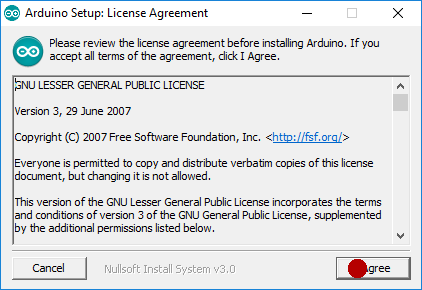
\includegraphics[width=0.9\textwidth]{figures/aride1.png}}
\item Selanjutnya akan muncul jendela `Arduino Setup: Installation Options'. Centang semua opsi yang ada, lalu klik `Next'.
\break
\centerline{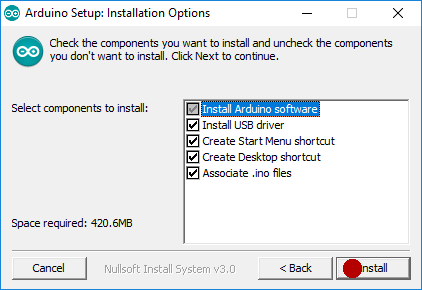
\includegraphics[width=0.9\textwidth]{figures/aride2.png}}
\item Setelah itu, akan muncul jendela `Arduino Setup: Installation Folder'. Kita diminta memilih folder instalasi Arduino.
\break
\centerline{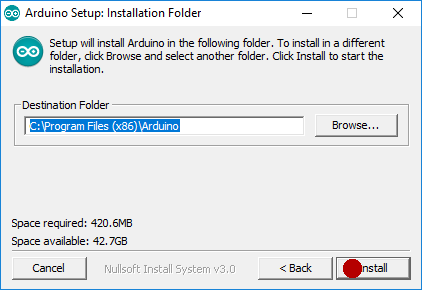
\includegraphics[width=0.9\textwidth]{figures/aride3.png}}
\item Selanjutnya proses instalasi akan dimulai.
\break
\centerline{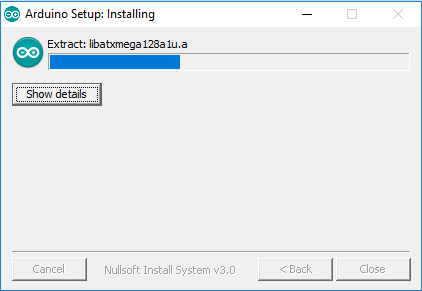
\includegraphics[width=0.9\textwidth]{figures/aride4.png}}
\item Pada saat melakukan proses instalasi, akan muncul jendela `Windows Security'. Jendela tersebut muncul apabila komputer kita belum terinstal driver - driver yang diperlukan. Klik tombol `Install'.
\break
\centerline{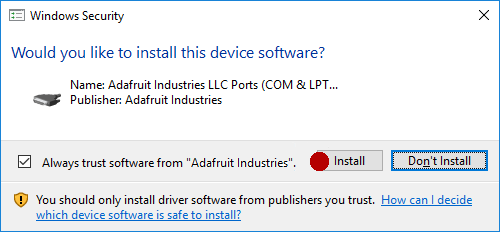
\includegraphics[width=0.9\textwidth]{figures/aride5.png}}
\break
\centerline{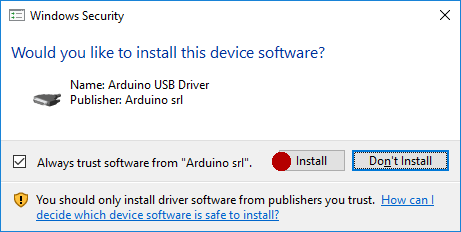
\includegraphics[width=0.9\textwidth]{figures/aride6.png}}
\break
\centerline{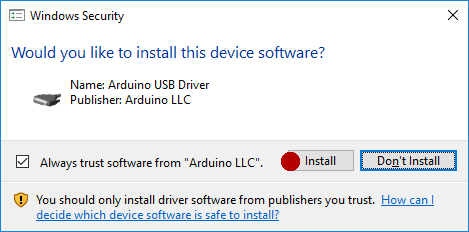
\includegraphics[width=0.9\textwidth]{figures/aride7.png}}
\item Selanjutnnya akan muncul jendela `Arduino Setup: Completed'. Jendela ini menandakan proses instalasi telah selesai. Klik tombol `Close'.
\break
\centerline{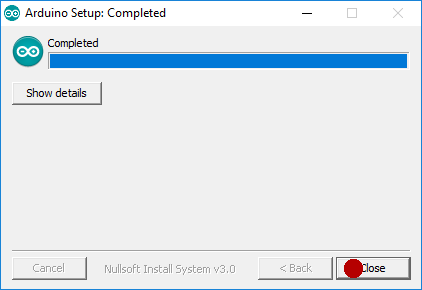
\includegraphics[width=0.9\textwidth]{figures/aride10.png}}
\item Setelah software IDE Arduino sudah terinstal. Coba cek di Start Menu Windows atau di desktop Anda, lalu jalankan aplikasi tersebut. Kemudian akan muncul splash screen seperti gambar di bawah ini.
\break
\centerline{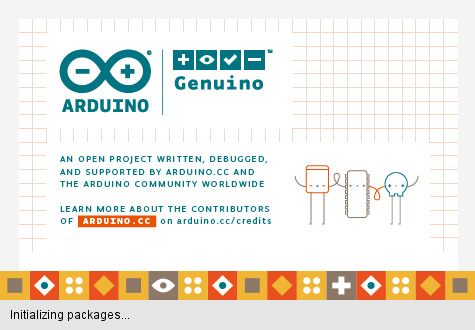
\includegraphics[width=0.9\textwidth]{figures/aride11.png}}
\item Selanjutnya akan muncul jendela IDE Arduino. Selamat Anda telah berhasil menginstal software IDE Arduino.
\break
\centerline{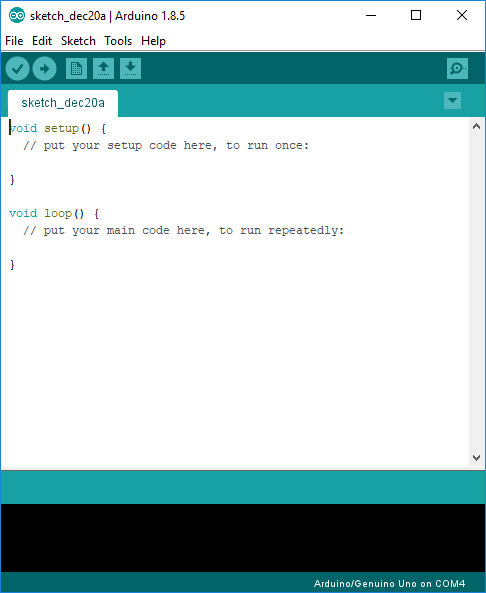
\includegraphics[width=0.9\textwidth]{figures/aride12.png}}
\end{enumerate}